\documentclass[12pt]{scrartcl}
\usepackage[sexy]{evan}
\usepackage[noend]{algpseudocode}
\usepackage{answers}
\usepackage{array}
\usepackage{tikz}
\newenvironment{allintypewriter}{\ttfamily}{\par}
\usepackage{listings}
\usetikzlibrary{arrows.meta}
\usepackage{color}
\usepackage[noend]{algpseudocode}
\newcommand{\U}{\mathcal{U}}
\newcommand{\E}{\mathbb{E}}
\usetikzlibrary{arrows}
\Newassociation{hint}{hintitem}{all-hints}
\renewcommand{\solutionextension}{out}
\renewenvironment{hintitem}[1]{\item[\bfseries #1.]}{}
\renewcommand{\O}{\mathcal{O}}
\declaretheorem[style=thmbluebox,name={Chinese Remainder Theorem}]{CRT}
\renewcommand{\theCRT}{\Alph{CRT}}
\setlength\parindent{0pt}
\usepackage{sansmath}
\usepackage{pgfplots}
\usetikzlibrary{automata}
\usetikzlibrary{positioning}  %                 ...positioning nodes
\usetikzlibrary{arrows}       %                 ...customizing arrows
\newcommand{\eqdef}{=\vcentcolon}
\usepackage[top=3cm,left=3cm,right=3cm,bottom=3cm]{geometry}
\newcommand{\mref}[3][red]{\hypersetup{linkcolor=#1}\cref{#2}{#3}\hypersetup{linkcolor=blue}}%<<<changed

\tikzset{node distance=4.5cm, % Minimum distance between two nodes. Change if necessary.
         every state/.style={ % Sets the properties for each state
           semithick,
           fill=cyan!40},
         initial text={},     % No label on start arrow
         double distance=4pt, % Adjust appearance of accept states
         every edge/.style={  % Sets the properties for each transition
         draw,
           ->,>=stealth',     % Makes edges directed with bold arrowheads
           auto,
           semithick}}


% Start of document.
\newcommand{\sep}{\hspace*{.5em}}


\begin{document}
\title{Design and Analysis of Algorithms \\ Section 0101}
\author{Ekesh Kumar\thanks{Email: \mailto{ekumar1@terpmail.umd.edu}}}
\date{\today}

\definecolor{dkgreen}{rgb}{0,0.6,0}
\definecolor{gray}{rgb}{0.5,0.5,0.5}
\definecolor{mauve}{rgb}{0.58,0,0.82}

\lstset{frame=tb,
  language=Java,
  aboveskip=3mm,
  belowskip=3mm,
  showstringspaces=false,
  columns=flexible,
  basicstyle={\small\ttfamily},
  numbers=none,
  numberstyle=\tiny\color{gray},
  keywordstyle=\color{blue},
  commentstyle=\color{dkgreen},
  stringstyle=\color{mauve},
  breaklines=true,
  breakatwhitespace=true,
  tabsize=3
}

\maketitle
These are my course notes for CMSC 451: Design and Analysis of Algorithms, taught by Professor Clyde Kruskal. Please e-mail corrections to \url{ekumar1@terpmail.umd.edu}

\tableofcontents


\newpage

\section{Tuesday, January 28, 2020}

\subsection{Introduction}

This is CMSC $451$: Design and Analysis of Algorithms. We will cover graphs, greedy algorithms, divide and conquer algorithms, dynamic programming, network flows, NP-completeness, and approximation algorithms.


\begin{itemize}
    \item Homeworks are due every other Friday or so; NP-homeworks are typically due every other Wednesday.
    \item There is a $25\%$ penalty on late homeworks, and there's one get-out-of-jail free card for each type of homework.
\end{itemize}

\subsection{Stable Marriage Problem}

As an introduction to this course, we'll discuss the \vocab{stable marriage problem}, which is stated as follows:

\begin{quote}
    Given a set of $n$ men and $n$ women, match each man with a woman in such a way that the matching is \textit{stable}.
\end{quote}

What do we mean when we call a matching is ``stable"? We call a matching \textit{unstable} if there exists some man $M$ who prefers a woman $W$ over the woman he is married to, and $W$ also prefers $M$ over the man she is currently married to. \\



In order to better understand the problem, let's look at the $n = 2$ case. Call the two men $M_1$ and $M_2$, and call the two women $W_1$ and $W_2$.

\begin{itemize}
    \item First suppose $M_1$ prefers $W_1$ over $W_2$ and $W_1$ prefers $M_1$ over $M_2$. Also, suppose that $M_2$ prefers $W_2$ over $W_1$ and $W_2$ prefers $M_2$, then 
    \item If both $W_1$ and $W_2$ prefer $M_1$ over $M_2$, and both $M_1$ and $M_2$ prefer $W_1$ over $W_2$, then it's still easy to see what will happen: $M_i$ will always match with $W_i$.
    \item Now let's say $M_1$ prefers $W_1$ to $W_2$, $M_2$ prefers $W_2$ to $W_1$, $W_1$ prefers $M_2$ to $M_1$, and $W_2$ prefers $M_1$ to $M_2$. In this case, the two men rank different women first, and the two women rank different men first. However, the men's preferences ``clash" with the women's preferences. One solution to this problem is to match $M_1$ with $W_1$ and $M_2$ with $W_2$. This is stable since both men get their top preference even though the two women are unhappy.
\end{itemize}

The solution to the problem starts to get a lot more complicated when the people's preferences do not exhibit any pattern. So how do we solve this problem in the general case? We can use the \vocab{Gale-Shapley algorithm}. Before discussing this algorithm, however, we can make the following observations about this problem:

\begin{itemize}
    \item Each of the $n$ men and $M$ woman are initially unmarried. If an unmarried man $M$ chooses the woman $W$ who is ranked highest on their list, then we cannot immediately conclude whether we can match $M$ and $w$ in our final matching.This is clearly the case since if we later find out about some other man $M_2$ who prefers $W$ over any other woman, $W$ may choose $M_2$ if she likes him more than $M$. However, we cannot immediately rule out  $M$ being matched to $W$ either since a man like $M_2$ may not ever come. 
    \item Just because everyone isn't happy doesn't mean a matching isn't stable. Some people might be unhappy, but there might not be anything they can do about it (if nobody wants to switch).
\end{itemize}


Moreover, we introduce the notion of a man \textit{proposing} to a woman, which a woman can either accept or reject. If she is already engaged and accepts a proposal, then her existing engagement breaks off (the previous man becomes unengaged).  \\


Now that we've introduced these basic ideas, we can now present the algorithm:


\vspace{1em}
\hline
\vspace{1em}

\begin{allintypewriter}
\# Input: A list of n men and n women to be matched. 

\hspace{0.5cm} 

\# Output: A valid stable matching.


\hspace{0.5cm}


stable\_matching \string{ 

\hspace{0.5cm} set each man and each woman to "free"

\hspace{0.5cm} while there exists a man m who still has a woman w to propose to \string{

\hspace{1cm} let w be the highest ranked woman m hasn't proposed to. 

\hspace{0cm}

\hspace{1cm} if w is free \string{ 

\hspace{1.5cm} (m, w) become engaged 

\hspace{1cm} \string} else \string{

\hspace{1.5cm} let m' be the man w is currently engaged to.

\hspace{1.5cm} if w prefers m' to m \string{ 

\hspace{2cm} (m', w) remain engaged. 

\hspace{1.5cm} \string} else \string{

\hspace{2cm} (m, w) become engaged and m' loses his partner.

\hspace{1.5cm} \string}

\hspace{1cm} \string}

\hspace{0.5cm} \string}

\string}

\end{allintypewriter}
\vspace{1em}
\hline
\vspace{1em}


\begin{proposition}
The Gale-Shapley algorithm terminates in $\mathcal{O}(n^2)$ time. 
\end{proposition}
\begin{proof}
In the worst case, $n$ men end up proposing to $n$ women. The act of proposing to another person is a constant-time operation. Thus, the $\mathcal{O}(n^2)$ runtime is clear.
\end{proof}%
\newpage
\section{Thursday, January 30, 2020}

\subsection{Optimality and Correctness of Gale-Shapley}


Last time, we introduced the Gale-Shapley algorithm to find a stable matching. Today, we'll prove that the algorithm is correct (i.e. it never produces an unstable matching), and it is optimal for men (i.e. the men always end up for their preferred choice). \\

First, we'll show that the algorithm is correct: \\

\begin{proposition}
The matching generated by the Gale-Shapley algorithm is never an unstable matching.  
\end{proposition}

\begin{proof}
Suppose, for the sake of contradiction, that $m$ and $w$ prefer each other over their current partner in the matching generated by the Gale-Shapley algorithm. This can happen either if $m$ never proposed to $w$, or if $m$ proposed to $w$ and $w$ rejected $m$. In the former case, $m$ must prefer his partner to $w$, which implies that $m$ and $w$ do not form an unstable pair. In the latter case, $w$ prefers her partner to $m$, which also implies $m$ and $w$ don't form an unstable pair. Thus, we arrive at a contradiction. 
\end{proof}

Next, we'll prove that the algorithm is optimal for men. However, before presenting the proof, observe that it is not too hard to see intuitively that the algorithm ``favors" the men. Since the men are doing all of the proposing and the women can only do the deciding, it turns out that the men always ends up with their most preferred choice (as long as the matching remains stable).

\begin{proposition}
The matching generated by the Gale-Shapley algorithm gives men their most preferred woman possible without contradicting stability. 
\end{proposition}

\begin{proof}
 \\



To see why this is true, let $A$ be the matching generated by the men-proposing algorithm, and suppose there exists some other matching $B$ that is better for at least one man, say $m_0$. If $m_0$ is matched in $B$ to $w_1$ which he prefers to his match in $A$, then in $A$, $m_0$ must have proposed to $w_1$ and $w_1$ must have rejected him. This can only happen if $w_1$ rejected him in favor of some other man --- call him $m_2$. This means that in $B$, $w_1$ is matched to $m_0$ but she prefers $m_2$ to $m_0$. Since $B$ is stable, $m_2$ must be matched to some woman that he prefers to $w_1$; say $w_3$. This means that in $A$, $m_2$ proposed to $w_3$ before proposing to $w_1$, and this means that $w_3$ rejected him. Since we can perform similar considerations, we end up tracing a ``cycle of rejections" due to the finiteness of the sets $A$ and $B$. 
\end{proof}



% Feb
\section{Tuesday, February 4, 2020}

Today, we'll recap graph terminology and elementary graph algorithms.

\subsection{Graph Terminology}

\begin{definition}
A \vocab{graph} $G = (V, E)$ is defined by a set of vertices $V$ and a set of edges $E$.
\end{definition}

The number of vertices in the graph, $|V|$, is the \vocab{order} of the graph, and the number of edges in the graph, $|E|$, is the \vocab{size} of the graph. Typically, we reserve the letter $n$ for the order of a graph, and we reserve $m$ for the size of a graph. 
\begin{definition}
We say a graph is \vocab{directed} if its edges can only be traversed in one direction. Otherwise, we say the graph is  \vocab{undirected}.
\end{definition}


\begin{definition}
A graph is called \vocab{simple} if it's an undirected graph without any loops (edges that start and end at the same vertex).
\end{definition}

\begin{definition}
A graph is \vocab{connected} if for every pair of vertices $u, v$, there exists a path between $u$ and $v$.
\end{definition}


\subsection{Graph Representations}

There are two primary ways in which we can represent graphs: \vocab{adjacency matrices} and \vocab{adjacency lists}. \\


An adjacency matrix is an $n\times n$ matrix \verb!A! in which \verb!A[u][v]! is equal to $1$ if the edge $(u, v)$ exists in the graph; otherwise, \verb!A[u][v]! is equal to $0$. Note that the adjacency matrix is symmetric if and only if the graph is undirected. \\

On the other hand, an adjacency list is a list of $|V|$ lists, one for each vertex. For each vertex $u \in V$, the adjacency list \verb!Adj[u]! contains all vertices $v$ for which there exists an edge $(u, v)$ in $E$. In other words, \verb!Adj[u]! contains all of the vertices adjacent to $u$ in $G$.  


Each graph representation has its advantages and disadvantages in terms of runtime. This is summarized by the table below.

\begin{figure}[h]
\centering
\begin{tabular}{ | m{2cm} | m{4cm}| m{4cm} | } 
\hline
 & \textsc{Adjacency List} & \textsc{Adjacency Matrix} \\ 
\hline
Storage  & $\mathcal{O}(n + m)$ & $\O(n^2)$ \\ 
\hline
Add vertex & $\mathcal{O}(1)$ & $\O(n^2)$ \\ 
\hline
Add edge & $\mathcal{O}(1)$ & $\O(1)$ \\ 
\hline
Remove vertex & $\mathcal{O}(n + m)$ & $\O(n^2)$ \\ 
\hline
Remove edge & $\mathcal{O}(m)$ & $\O(1)$ \\ 
\hline
\end{tabular}
\caption{Adjacency Matrix vs Adjacency List}
\end{figure}

An explanation of these runtimes are provided below:

\begin{itemize}
    \item An adjacency list requires $\O(n + m)$ since there are $n$ lists inside of the adjacency list. Now for each vertex $v_i$, there are $\text{deg}(v_i)$ vertices in the $i^{\text{th}}$ adjacency list. Since $\sum_{i} \text{deg}(v_i) = \O(m)$, we conclude that the adjacency list representation of a graph requires $\O(n + m)$ space. On the other hand, the adjacency matrix representation of a graph requires $\mathcal{O}(n^2)$ space since we are storing an $n\times n$ matrix. 
    \item We can add a vertex in constant time in an adjacency list by simply inserting a new list into the adjacency list. On the other hand, to insert a new vertex in an adjacency matrix, we need to increase the dimensions of the adjacency matrix from $n\times n$ to $(n + 1) \times (n + 1)$. This requires $\mathcal{O}(n^2)$ time since we need to copy over the old matrix to a new matrix.
    \item We can insert an edge $(u, v)$ into an adjacency list in constant time by simply appending $v$ to the end of $u$'s adjacency list (and $u$ to the end of $v$'s adjacency list if the graph is undirected). Similarly, we can insert an edge in an adjacency matrix in constant time by setting \verb!A[u][v]! to $1$ (and also seting \verb!A[v][u]! to $1$ if the graph is undirected). 
    \item Removing a vertex requires $\mathcal{O}(n + m)$ time in an adjacency list since we need to traverse the entire adjacency list and remove any incoming our outgoing edges to the vertex being removed. Similarly, this operation takes $\O(n^2)$ time in an adjacency matrix since we need to traverse the entire matrix to remove incoming and outgoing edges.
    \item Removing an edge $(u, v)$ requires $\mathcal{O}(m)$ time in an adjacency matrix since we only need to search the adjacency lists of $u$ and $v$ (in the worst case, these vertices have all $m$ edges in their adjacency list). On the other hand, this operation takes constant time in an adjacency matrix since we're just setting \verb!A[u][v]! to $0$.
\end{itemize}


\subsection{Graph Traversal}

Before discussing recapping the two primary types of graph traversal, we will introduce some more terminology. \\

\begin{definition}
A \vocab{connected component} of a graph is a maximially connected subgraph of $G$. Each vertex belongs to one connected component as does each edge.
\end{definition}

There are two primary ways in which we can traverse graphs: using \vocab{breadth-first search} or \vocab{depth-first search}. These two methods of graph traversal are very similar, and they allow us to explore every vertex in a connected components of a graph. 


\begin{enumerate}
    \item Breadth-first search starts at some source vertex $v$ and all vertices with distance $k$ away from $v$ before visiting vertices with distance $k + 1$ from $v$. This algorithm is typically implemented using a queue, and it can be used to find the shortest path (measured by the number of edges) from the source vertex.
    \item Depth-first search starts from a source vertex and keeps on going outward until we cannot proceed any further. We must subsequently backtrack and begin performing the depth-first search algorithm again.  This algorithm is typically implemented using a stack, whether it be the data structure or the function call stack.
\end{enumerate}

Both of these algorithms run in $\O(n^2)$ time on an adjacency matrix and $\O(n + m)$ time on an adjacency list. \\

Since breadth-first search and depth-first search are guaranteed to visit all of the vertices in the same connected component as the starting vertex, we can easily write an algorithm that counts the number of connected components in a graph. \\

Some C++ code is provided below.

\begin{lstlisting}
/* visited[] is a global Boolean array. */
/* AdjList is a global vector of vectors. */
void dfs(int v) {
    visited[v] = true;
    for (int i = 0; i < AdjList[v].size(); i++) {
        int u = AdjList[v][i];
        if (!visited[u]) {
            dfs(v);
        }
    }
}

int main(void) {
    /* Assume AdjList and other variables have been declared. */
    int numCC = 0;
    for (int i = 0; i < num_vertices; i++) {
        if (!visited[i]) {
            numCC = numCC + 1;
            dfs(i);
        }
    }
}
\end{lstlisting}
\newpage
\section{Thursday, February 6, 2020}

Today, we'll discuss algorithms to find articulation points and biconnected components. 

\subsection{Articulation Points}

\begin{definition}
An \vocab{articulation point} or \vocab{cut vertex} is a vertex in a graph $G = (V, E)$ whose removal (along with any incident edges) would disconnect $G$. 
\end{definition}

\begin{definition}
A graph is said to be \vocab{biconnected} if the graph not have any articulation points. 
\end{definition}

For example, consider the following graph:

\begin{figure}[h]
\centering
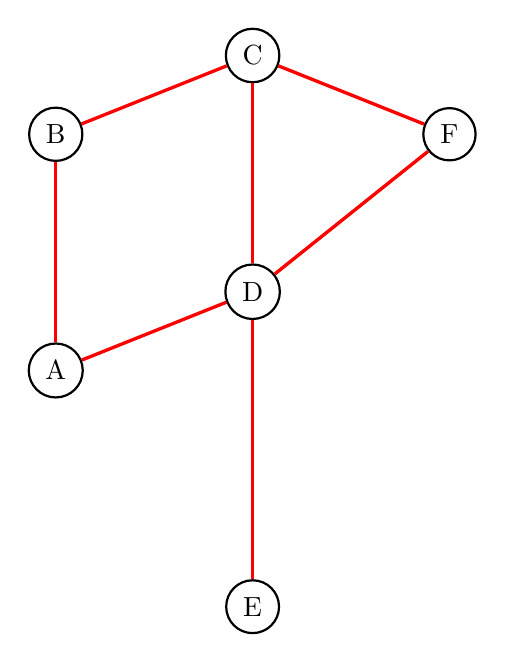
\begin{tikzpicture}
\begin{scope}[every node/.style={circle,thick,draw}]
    \node (A) at (0,0) {A};
    \node (B) at (0,3) {B};
    \node (C) at (2.5,4) {C};
    \node (D) at (2.5,1) {D};
    \node (E) at (2.5,-3) {E};
    \node (F) at (5,3) {F} ;
\end{scope}

\begin{scope}[>={Stealth[black]},
              every node/.style={fill=white,circle},
              every edge/.style={draw=red,very thick}]
    \path [-] (A) edge (B);
    \path [-] (B) edge (C);
    \path [-] (A) edge (D);
    \path [-] (D) edge (C);
    % \path [-] (A) edge (E);
    \path [-] (D) edge (E);
    \path [-] (D) edge (F);
    \path [-] (C) edge (F);
    % \path [-] (E) edge (F); 
    % \path [-] (B) edge[bend right=40] (F); 
\end{scope}
\end{tikzpicture}
\caption{A Graph with an Articulation Point}
\end{figure}

In the diagram above, Vertex $D$ is an articulation point. To see why, note that if we were to remove Vertex $D$ (and any incident edges to $D$) from the graph, then we would end up with two connected components: the first component would contain the vertices $A, B, C,$ and $F$, whereas the second component would only contain the vertex $E$. \\

Why are articulation points important? One example in which searching for articulation points is important is in the study of networks. In a network modeled by a graph, an articulation point represents a vulnerability: it is a single point whose failure would split the network into two or more components (preventing communication between the nodes in different networks). 
 \\
 
 
 How do we find an articulation points? The brute force algorithm is as follows:
 
 \begin{enumerate}
     \item Run an $\mathcal{O}(V + E)$ depth-first search or breadth-first search to count the number of connected components in the original graph $G = (V, E)$. 
     \item For each vertex $v\in V$, remove $v$ from $G$, and remove any of $v$'s incident edges. Run an $\mathcal{O}(V + E)$ depth-first search or breadth-first search again, and check if the number of connected components increases. If so, then $v$ is an articulation point. Restore $v$ and any of its incident edges.
 \end{enumerate}
 
This naive algorithm calls the depth-first search or breadth-first search algorithm $\mathcal{O}(V)$ times. Hence, it runs in $\mathcal{O}(V \times (V + E)) = \mathcal{O}(V^2 + VE)$ time. \\
 
 
While this algorithm \textit{works}, it is not as efficient as we can get. We will now describe a linear-time algorithm that runs the depth-first search algorithm just \textit{once} to identify all articulation points and bridges. This algorithm is often accredited to Hopcraft and Tarjan. \\
 
 
In this modified depth-first search, we will now maintain two numbers for each vertex $v$: \verb!dfs_num(v)! and \verb!dfs_low(v)!. The quantity \verb!dfs_num(v)! represents a label that we will assign to nodes in an increasing fashion. For instance, the vertex from which we call depth-first search would have a \verb!dfs_num! of $0$. The subsequent vertex we visit would be assigned a \verb!dfs_num! of $1$, and so on. \\
 
On the other hand, the quantity \verb!dfs_low(v)!, also known as the \vocab{low-link value} of the vertex $v$, represents the smallest \verb!dfs_num! reachable from that node while performing a depth-first (including itself). \\
 
Here's an example. Consider the following directed graph: 
  
  
\begin{figure}[h]
\centering
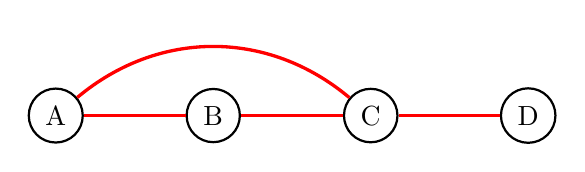
\begin{tikzpicture}
\begin{scope}[every node/.style={circle,thick,draw}]
    \node (A) at (0,0) {A};
    \node (B) at (2,0) {B};
    \node (C) at (4,0) {C};
    \node (D) at (6,0) {D};
    % \node (E) at (2.5,-3) {E};
    % \node (F) at (5,3) {F} ;
\end{scope}

\begin{scope}[>={Stealth[black]},
              every node/.style={fill=white,circle},
              every edge/.style={draw=red,very thick}]
    \path [-] (A) edge (B);
    \path [-] (B) edge (C);
    \path [-] (C) edge (D);
    \path [-] (C) edge[bend right=40] (A); 

    % \path [-] (A) edge (D);
    % \path [-] (D) edge (C);
    % \path [-] (A) edge (E);
    % \path [-] (D) edge (E);
    % \path [-] (D) edge (F);
    % \path [-] (C) edge (F);
    % \path [-] (E) edge (F); 
    % \path [-] (B) edge[bend right=40] (F); 
\end{scope}
\label{artpoint:ex}
\end{tikzpicture}
\caption{Articulation Point Example}
\end{figure}

Suppose we perform a depth-first search starting at Vertex $A$. 

\begin{itemize}
    \item Vertex $A$ will be assigned a \verb!dfs_num! of $0$ since this is the first vertex that we're visiting. Moreover, $0$ is the smallest \verb!dfs_num! that is reachable from $A$ (all other vertices have their \verb!dfs_num! set to \verb!nil! or \verb!INFINITY!). Hence, we set \verb!dfs_num(A) = 0! and \verb!dfs_low(A) = 0!. 
    \item Next, we visit vertex $B$. Vertex $B$ is assigned a \verb!dfs_num! of $1$ since it's the second vertex we're visiting. Moreover, Vertex $B$ has a \verb!dfs_low! value of $0$ since we can reach a vertex with a \verb!dfs_num! value of $0$ through the path $B \rightarrow C \rightarrow A$. Note that it would be invalid to say that the path $B \rightarrow A$ causes \verb!dfs_low(B)! to equal $0$ since we cannot go backwards in the depth-first search traversal. 
    \item Applying similar reasoning, we find that vertex $C$ ends up with a \verb!dfs_num! value of $2$, and it also has a \verb!dfs_low! value of $0$ (we can reach vertex $A$).
    \item Finally, vertex $B$ ends up with a \verb!dfs_num! value of $3$; however, no vertices with a lower \verb!dfs_num! value are reachable from $D$. Hence, the \verb!dfs_low! value of $D$ is also equal to $3$. Note that it is incorrect to say that $D$ has a \verb!dfs_low! value of $0$ through the path $D\rightarrow C\rightarrow A$ since we cannot revisit vertices while performing the depth-first search algorithm. 
\end{itemize}


Why do we care about these \verb!dfs_num! and \verb!dfs_low! values? It becomes more clear when we consider the depth-first search tree produced by calling the depth-first search algorithm. The quantity \verb!dfs_low(v)! represents the smallest \verb!dfs_num! value reachable from the current depth-first search spanning subtree rooted at the vertex $v$.  The value \verb!dfs_low(v)! can only be made smaller if there's a back edge (an edge from a vertex $v$ to an ancestor of $v$) in the depth-first search tree. \\

This leads us to make the following observation: If there's a vertex $u$ with neighbor $v$ satisfying \verb!dfs_low(v) >= dfs_num(u)!, then we can conclude that vertex $u$ is an articulation point.  Note that this makes sense intuitively since it means that the \textit{smallest} numbered vertex that we can ever reach starting from vertex $v$ is greater than or equal to the number we assigned to $u$. Hence, removing $u$ would disconnect \verb!v! from any vertex with smaller \verb!dfs_num! than \verb!dfs_num(u)!. \\


Going back to the previous graph figure, we can note that the following:
\[
\verb!3 = dfs_num(D) >= dfs_low(C) = 0!
\]
As stated previously, this implies that Vertex $C$ is an articulation point. Note that removing Vertex $C$ would disconnect the vertices $A$ and $B$ from Vertex $D$.  \\

Now, there's one special case to this algorithm. The root of the depth-first search spanning tree (the vertex that we choose as the source in the first depth-first search call) is an articulation point only if it has more than one children. This one case is not detected by the algorithm; however, it is easy to check in implementation. \\

% When actually implementing the algorithm, we can assign \verb!dfs_num! values ``on-the-fly" when we visit the vertex. A C++ implementation is provided below: \\

% \begin{lstlisting}
% int dfsCounter; /* Used to assign vertices their dfs_num value. */
% int dfs_num[10000]; /* Stores the dfs_num values of each vertex. */
% int dfs_lo[10000]; /* Stores the dfs_low values of each vertex. */
% int color[10000]; /* Check if we've visited the vertex yet. */
% int parent[10000]; /* We maintain the parent of a vertex so we don't update the dfs_low value with an already-visited vertex. */
% bool isArticulationPoint[10000];


% /* O(V + E) Articulation Point Algorithm. */
% void dfs(int u, const vector<vector<int>>& AdjList) {
%   color[u] = 1;
%   dfs_num[u] = dfs_lo[u] = dfsCounter++;
  
%   for (int i = 0; i < AdjList[u].size(); i++) {
%     int v = AdjList[u][i];
%     if (!visited[v]) {
%       /* Vertex v hasn't been visited. */
%       parent[v] = u;
%       dfs(v, AdjList);

%       if (dfs_lo[v] >= dfs_num[u]) {
%         // Vertex u is an articulation point. 
%         isArticulationPoint[u] = true;
%       }
%       /* Update the dfs_lo value of u. */
%       dfs_lo[u] = MIN(dfs_lo[u], dfs_lo[v]);
%     } else if (color[v] == 1 && parent[u] != v) {
%       /* (u, v) is a back edge in the depth-first search tree. */
%       /* We've already visited vertex v, so we just update the dfs_lo value. */
%       dfs_lo[u] = min(dfs_lo[u], dfs_num[v]);
%     }
%   }
%   color[u] = 2;
% }
% \end{lstlisting}



\end{document}




